\section{Research Timetable}\label{sec:timetable}

\begin{itemize}
    \item Talk about thesis structure.
    \item Derive tasks from structure.
    \item Given brief overview of the task scheduling.
\end{itemize}

This section aims to outline how the remaining time in the PhD will be
allocated.
In Section \ref{sec:structure}, the structure for the PhD Thesis was proposed.
This structure lends itself to three phases of research, each pertaining to an
objective:
\begin{itemize}
    \item Objective 1: exploring the Ensemble Kalman Filter with a simple ABM.
    \item Objective 2: comparing the effectiveness of the Ensemble Kalman Filter
        when applied to different models.
    \item Objective 3: comparing the effectiveness of the Ensemble Kalman Filter
        with other data assimilation methods.
\end{itemize}
These objectives are timetabled as shown in the Gantt chart in Figure
\ref{fig:gantt_chart}.
The Gantt chart also proposes some of the conference that may be attended to
present parts of the research; GISRUK in the Spring of 2020 would provide the
opportunity to present the results of Objective 1, SIMSOC in the Autumn of 2020
would provide the opportunity to present the results of Objective 2 and SIMSOC
in the Autumn of 2021 would provide the opportunity to present the results of
Objective 3.
Subsequent RSG meetings are also expected to fall approximately around the end
of each of the Objectives.

\begin{figure}[h!]
    \centering
    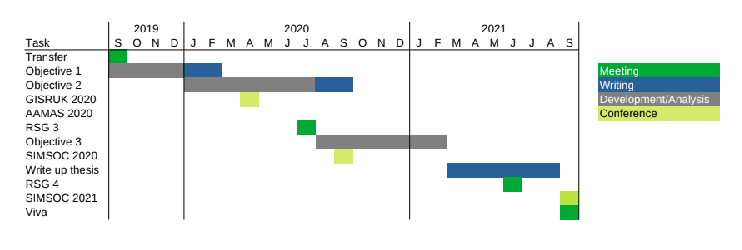
\includegraphics[width=\textwidth]{gantt_chart.eps}
    \caption{Gantt chart outline allocation of time over next two
    years.}\label{fig:gantt_chart}
\end{figure}
